\lecture{10}{11.08.2020}{Lyapunov Stability}

The major point we are concerned is how to assess the stability of a nonlinear system. That is, nonlinear analysis.

Nonlinear analysis is advantageous as linearization is an approximation and, therefor, valid only for small perturbations/signals.

To assess the stability, it is important to be able to prove mathematically/analytically that a given system remains stable under nonlinear behavior for large signals.

\subsection*{Definitions}

Given a not-necessarily-linear system \[
    \dot{x}(t) = f\left( x(t) \right) 
\] an equilibrium point $\overline{x}$ is a solution to \[
f\left( \overline{x}(t) \right) = 0 \forall t>\overline{t}
\]. An equilibrium point is calculated by solving \[
    f\left( \overline{x} \right) = 0
\] as it means that the derivative of the input is null and, therefore, the input achieves a constant value.

\begin{description}
    \item[Stability] is achieved if a given equilibrium point $\overline{x}$ if, for any perturbation of the system in a neighborhood of $\overline{x}$ results in a trajectory that remains in a finite neighborhood (epsilon-delta limit definition).
    \item[Asymptotical Stability] is achieved when it is stable and any resulting trajectory of neighbor perturbations of $\overline{x}$ converges to the equilibrium point (0).
\end{description}
Note that attractiveness does not imply stability.

\begin{figure}[H]
    \centering
    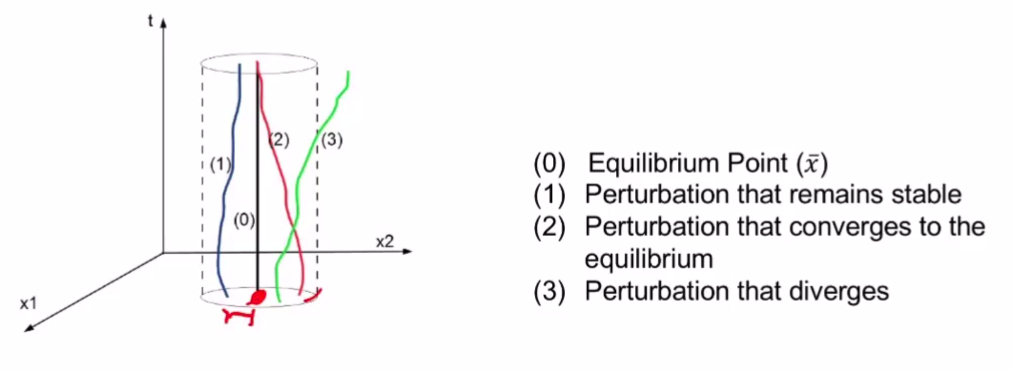
\includegraphics[width=0.8\textwidth]{figures/equilibrium_point.png}
    \caption{Equilibrium point demonstration. Note the axis.}
    \label{fig:figures-equilibrium_point-png}
\end{figure}

\subsection*{Lyapunov Method}

It consists in defining a scalar function $V\left( x \right) $ based on the state variables and to prove that this function is decreasing along the system trajectories. Based upon positive/negative definite function.

\begin{figure}[h!]
    \centering
    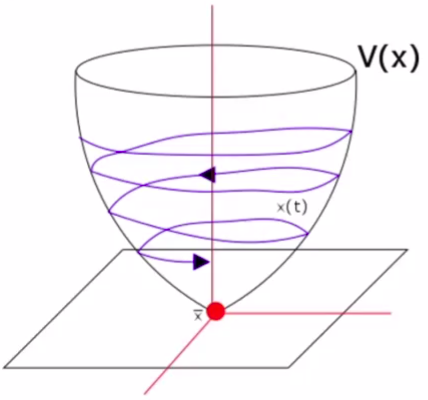
\includegraphics[width=0.8\textwidth]{figures/lyapunov_function.png}
    \caption{Lyapunov function illustrated.}
    \label{fig:figures-lyapunov_function-png}
\end{figure}

\begin{description}
    \item[Positive definite] is a function $V\left( x \right) :R^{n}\to R$ that, in a point $\overline{x}$ is guaranteed that $V\left( \overline{x} \right) =0$ and  $\exists \xi>0:V\left( x \right) >0 \forall x:\|x-\overline{x}\|<\xi$ when $x\neq \overline{x}$ (if we relax the restriction on the neighborhood of $\overline{x}$ to $V(x) \ge 0$, then this function is \textbf{semi positive-definite}).
    \item[Negative definite] is a function $V\left( x \right) :R^{n}\to R$ such that $-V(x)$ is \emph{positive definite}.
\end{description}

Usually it is very difficult for nonlinear systems to prove behavior over the entire design space, so what is normally assessed is the region where perturbations develop towards the equilibrium point (attraction zone).

Now on equilibrium points, note that the definition of stability is related to the size of the perturbation. As in the example in figure \ref{fig:figures-lyapunov_equilibrium_points-png}, note that both points 1 and 2 are equilibrium points, but point 2 is asymptotically stable if the perturbation is small enough. If the perturbation is larger than the distance from 2 to 1, for example, even point 2 is unstable.

\begin{figure}[h]
    \centering
    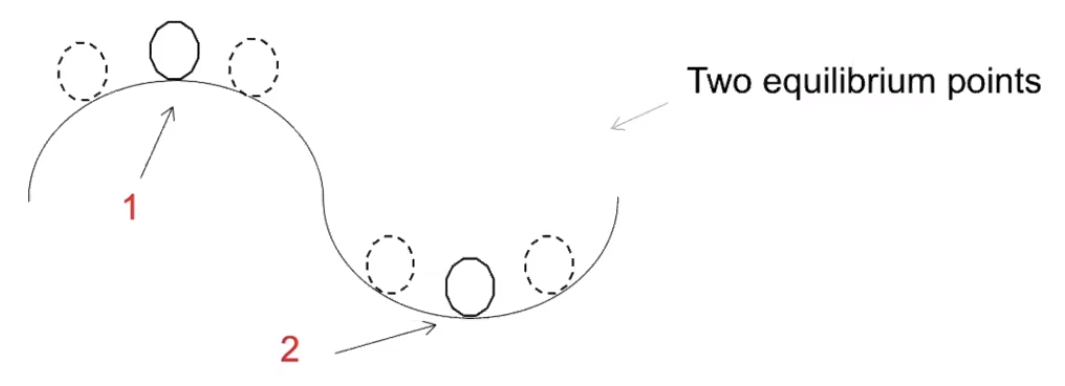
\includegraphics[width=0.8\textwidth]{figures/lyapunov_equilibrium_points.png}
    \caption{Equilibrium points example}
    \label{fig:figures-lyapunov_equilibrium_points-png}
\end{figure}

Given a system $\dot{x}(t)=f\left( x(t) \right) $, we define a Lyapunov function $V\left( x \right) $ such that
\begin{itemize}
    \item $V$ is a \emph{positive-definite} function over $x$.
    \item $\frac{d}{dt}V\left( x \right) =\dot{V}\left( x \right)$ is \emph{(semi) negative-definite}.
	\begin{itemize}
	    \item if strictly negative-definite, then \emph{asymptotic stability} is achieved, that is, effectively an attraction zone.
	    \item if semi negative-definite, then some \emph{oscillations} will occur around the equilibrium point in the case of $\frac{d}{dt}V = 0$.
	\end{itemize}
\end{itemize}

Note that the Lyapunov method defines only a sufficient condition, which means that if the test fails, that is, we cannot determine V characteristics, it does not imply in instability. Of course it builds a suspect, but it is not a necessary condition for stability.

As this function is not previously defined, we must search for it in the application. The energy function is a useful candidate, as it is of use to observe the relation between kinetic and potential energy in the surface of a system. Observe this relation in the example in figure \ref{fig:figures-lyapunov_equilibrium_points-png}.

\begin{description}
    \item[Kinetc Energy] from classical mechanics, is defined as $E_k = \frac{1}{2}mv^{2}$, which we could use, given a system $\dot{x}(t)=f\left( x(t) \right) $, as $E_k(t)=\frac{1}{2}\dot{x}^{2}(t)$
    \item[Potential Energy] defined as $U=\frac{1}{2}kx^{2}$ (elastic energy) could be used as \[
    V(x(t))=\frac{1}{2}x^{2}(t)
    \] which would imply in \[
    \frac{\partial V}{\partial t} (t)=\frac{\partial V}{\partial x} \frac{\partial x}{\partial t} (t)=x(t)\dot{x}(t)=x(t)f\left( x(t) \right) 
    \] 
\end{description}

\subsubsection*{Example}

Given a system defined by \[
\dot{x}(t)=ax(t)
\] we would like to see for which values of $a$ the system is asymptotically stable.

We now that the solution of such a system is of the form \[
x(t)=x_0\exp^{at}
\], so the solution for it to converge to a equilibrium point at 0 would be $a<0$. But we can also verify this using a Lyapunov function defined by the quadratic function \[
V(x) = \frac{x^{2}}{2}
\], so at the equilibrium point $x(t)=0$, we have $V(x)\ge 0$ and \[
\frac{\partial V}{\partial t}(t) =\frac{\partial V}{\partial x} \frac{\partial x}{\partial t}(t) = \frac{2x(t)}{2}\dot{x}(t) = ax^{2}(t)
\] which gives us the same result, that is, $a<0\implies V$ is negative definite, therefore, the system is asymptotically stable based on Lyapunov criteria. But it does not tell us anything for $a>0$!

\subsection*{Introduction to Linearization}

Even though so far we have seen the application for systems of the form \[
\dot{x}(t)=f\left( x(t) \right) 
\], the theory is easily extensible to time dependant systems with inputs of the form \[
\dot{x}(t)=f\left( x(t),u(t) \right) 
\] which, in a closed-loop, would be \[
\dot{x}(t)=f\left( x(t),g\circ x(t) \right) 
\], $g$ being the control function.

Through the $g$ function, we can map the closed-loop system in a new system \[
\dot{x}^{*}(t)=h\left( x^{*}(t) \right) 
\] that has \textbf{reduced complexity} and \textbf{new and well defined characteristics}. The ultimate goal is to achieve a new system \[
\dot{x}^{*}(t)=Ax^{*}(t)
\] stable and robust, in which $A$ is time-invariant.

The theories to perform this operation are all based on restricting the state variables to move on a manifold $\psi(x)=0$. For this, there are two challenges that occur
\begin{itemize}
    \item Reaching the manifold from any initial condition on the state space.
    \item Stability on the manifold.
\end{itemize}
One basic example is in a two dimensional state space, defining a linear manifold \[
    \psi(x) = a^{T}x + c = 0
\], in which a is a vector, thus reducing the dimension of the system by one degree.

In this situation, it is very common to define the Lyapunov function as a quadratic function of the manifold, so \[
    V(x) = \frac{1}{2}\psi^{2}(x)
\], which implies in \[
\dot{V}=\psi \dot{\psi}
\].
